\documentclass{article}
\usepackage{tikz}
\usepackage{amssymb}
\pagestyle{empty}
\begin{document}
% GEOMIRA export: TikZ. One unit is 25bp (33.333333 px on screen).
% Needs \usepackage{tikz} and \usepackage{amssymb}.
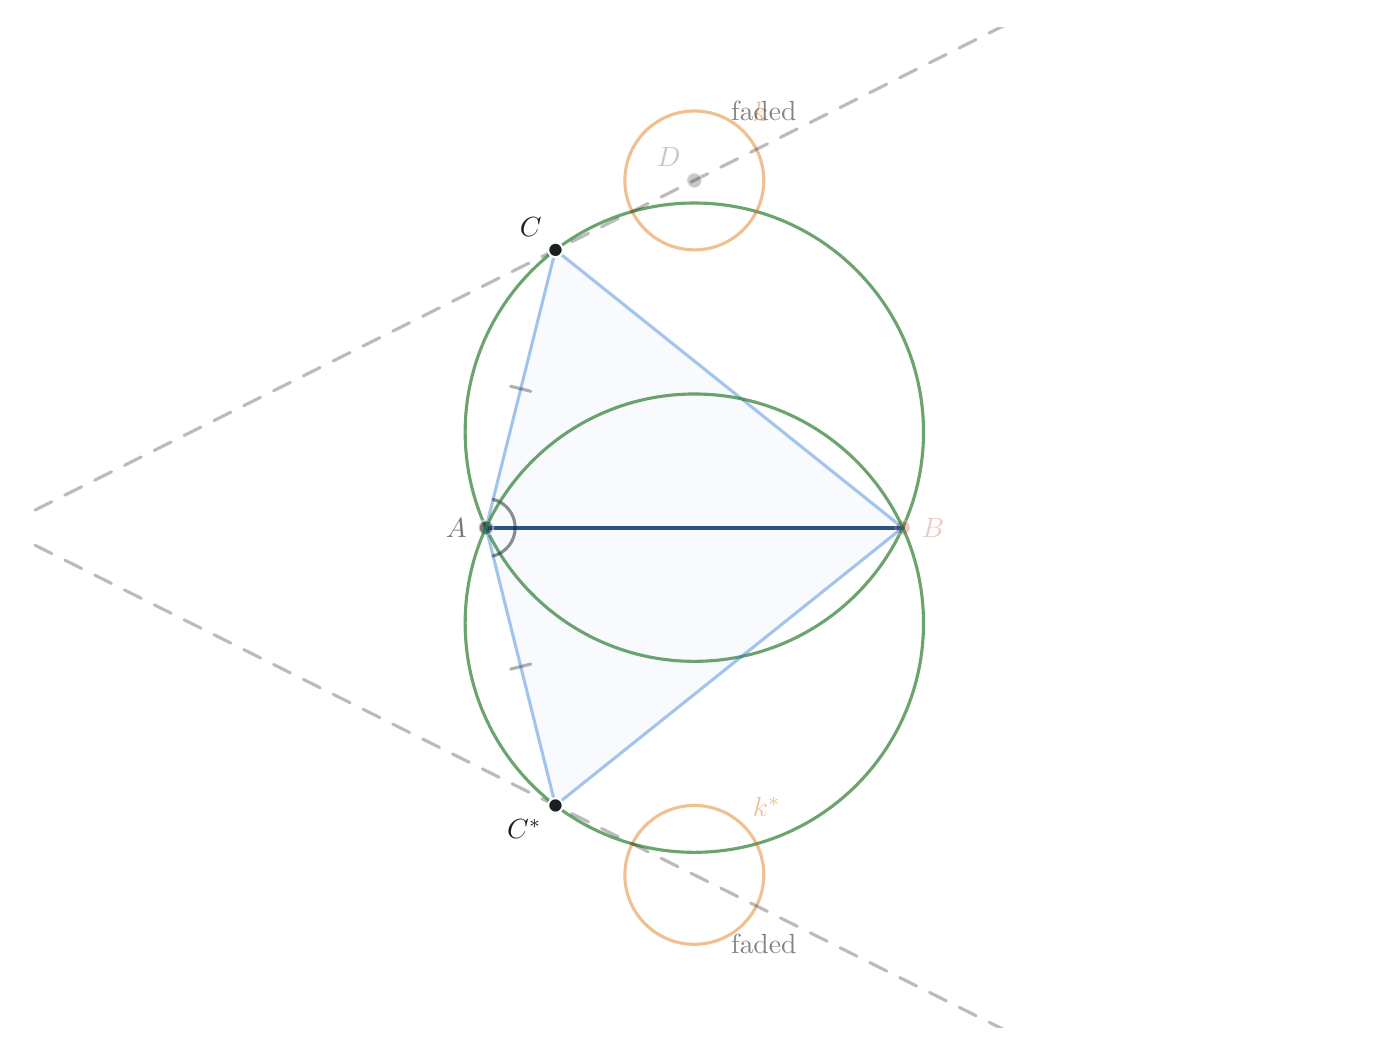
\begin{tikzpicture}[x=25bp, y=25bp, line cap=round, line join=round]
\definecolor{gmc0}{HTML}{1F6FD1}
\definecolor{gmc1}{HTML}{2E7D32}
\definecolor{gmc2}{HTML}{D9730D}
\definecolor{gmc3}{HTML}{1B1F24}
\definecolor{gmc4}{HTML}{FBFBF8}
\definecolor{gmc5}{HTML}{B3261E}
\clip (-6.6,-7.2) rectangle (12.6,7.2);
% tri
\fill[gmc0, fill opacity=0.032] (0,0) -- (6,0) -- (1,4) -- cycle;
\draw[gmc0, line width=1.125bp, draw opacity=0.4] (0,0) -- (6,0);
\draw[gmc0, line width=1.125bp, draw opacity=0.4] (6,0) -- (1,4);
\draw[gmc0, line width=1.125bp, draw opacity=0.4] (1,4) -- (0,0);
% ω
\draw[gmc1, line width=1.125bp, draw opacity=0.7] (6.3001,1.375) arc[start angle=0, end angle=360, radius=3.30009];
% k
\draw[gmc2, line width=1.125bp, draw opacity=0.45] (4,5) arc[start angle=0, end angle=360, radius=1];
% ab
\draw[gmc3, line width=1.5bp, draw opacity=0.8] (0,0) -- (6,0);
% l
\draw[gmc3, line width=1.125bp, dash pattern=on 6.75bp off 5.25bp, draw opacity=0.3] (-8.64,-0.82) -- (11.48,9.24);
% m1
\draw[gmc3, line width=1.125bp, draw opacity=0.35] (0.3545,2.0364) -- (0.6455,1.9636);
% a1
\draw[gmc3, line width=1.125bp, draw opacity=0.5] (0.42,0) arc[start angle=0, end angle=75.9638, radius=0.42];
% A
\filldraw[fill=gmc3, draw=gmc4, line width=0.75bp, opacity=0.6] (0,0) circle[radius=2.625bp];
% B
\filldraw[fill=gmc5, draw=gmc4, line width=0.75bp, opacity=0.25] (6,0) circle[radius=2.625bp];
% C
\filldraw[fill=gmc3, draw=gmc4, line width=0.75bp] (1,4) circle[radius=2.625bp];
% t1
% D
\filldraw[fill=gmc3, draw=gmc4, line width=0.75bp, opacity=0.25] (3,5) circle[radius=2.625bp];
% tri*
\fill[gmc0, fill opacity=0.032] (0,0) -- (6,0) -- (1,-4) -- cycle;
\draw[gmc0, line width=1.125bp, draw opacity=0.4] (0,0) -- (6,0);
\draw[gmc0, line width=1.125bp, draw opacity=0.4] (6,0) -- (1,-4);
\draw[gmc0, line width=1.125bp, draw opacity=0.4] (1,-4) -- (0,0);
% ω*
\draw[gmc1, line width=1.125bp, draw opacity=0.7] (6.3001,-1.375) arc[start angle=0, end angle=360, radius=3.30009];
% k*
\draw[gmc2, line width=1.125bp, draw opacity=0.45] (4,-5) arc[start angle=0, end angle=360, radius=1];
% l*
\draw[gmc3, line width=1.125bp, dash pattern=on 6.75bp off 5.25bp, draw opacity=0.3] (-8.64,0.82) -- (11.48,-9.24);
% m1*
\draw[gmc3, line width=1.125bp, draw opacity=0.35] (0.6455,-1.9636) -- (0.3545,-2.0364);
% a1*
\draw[gmc3, line width=1.125bp, draw opacity=0.5] (0.1019,-0.4075) arc[start angle=-75.9638, end angle=0, radius=0.42];
% C*
\filldraw[fill=gmc3, draw=gmc4, line width=0.75bp] (1,-4) circle[radius=2.625bp];
% t1*
\node[anchor=south west, inner sep=0pt, text=gmc2, text opacity=0.45] at (3.8344,5.8344) {$k$}; % label of k
\node[anchor=east, inner sep=0pt, text=gmc3, text opacity=0.6] at (-0.27,0) {$A$}; % label of A
\node[anchor=west, inner sep=0pt, text=gmc5, text opacity=0.25] at (6.27,0) {$B$}; % label of B
\node[anchor=south east, inner sep=0pt, text=gmc3] at (0.8091,4.1909) {$C$}; % label of C
\node[anchor=center, inner sep=0pt, text=gmc3, text opacity=0.55] at (4,6) {faded}; % label of t1
\node[anchor=south east, inner sep=0pt, text=gmc3, text opacity=0.25] at (2.8091,5.1909) {$D$}; % label of D
\node[anchor=south west, inner sep=0pt, text=gmc2, text opacity=0.45] at (3.8344,-4.1656) {$k^{*}$}; % label of k*
\node[anchor=north east, inner sep=0pt, text=gmc3] at (0.8091,-4.1909) {$C^{*}$}; % label of C*
\node[anchor=center, inner sep=0pt, text=gmc3, text opacity=0.55] at (4,-6) {faded}; % label of t1*
\end{tikzpicture}

\end{document}
